% !TEX root = ../main.tex
    \begin{figure}[b!]
        \centering\frame{
        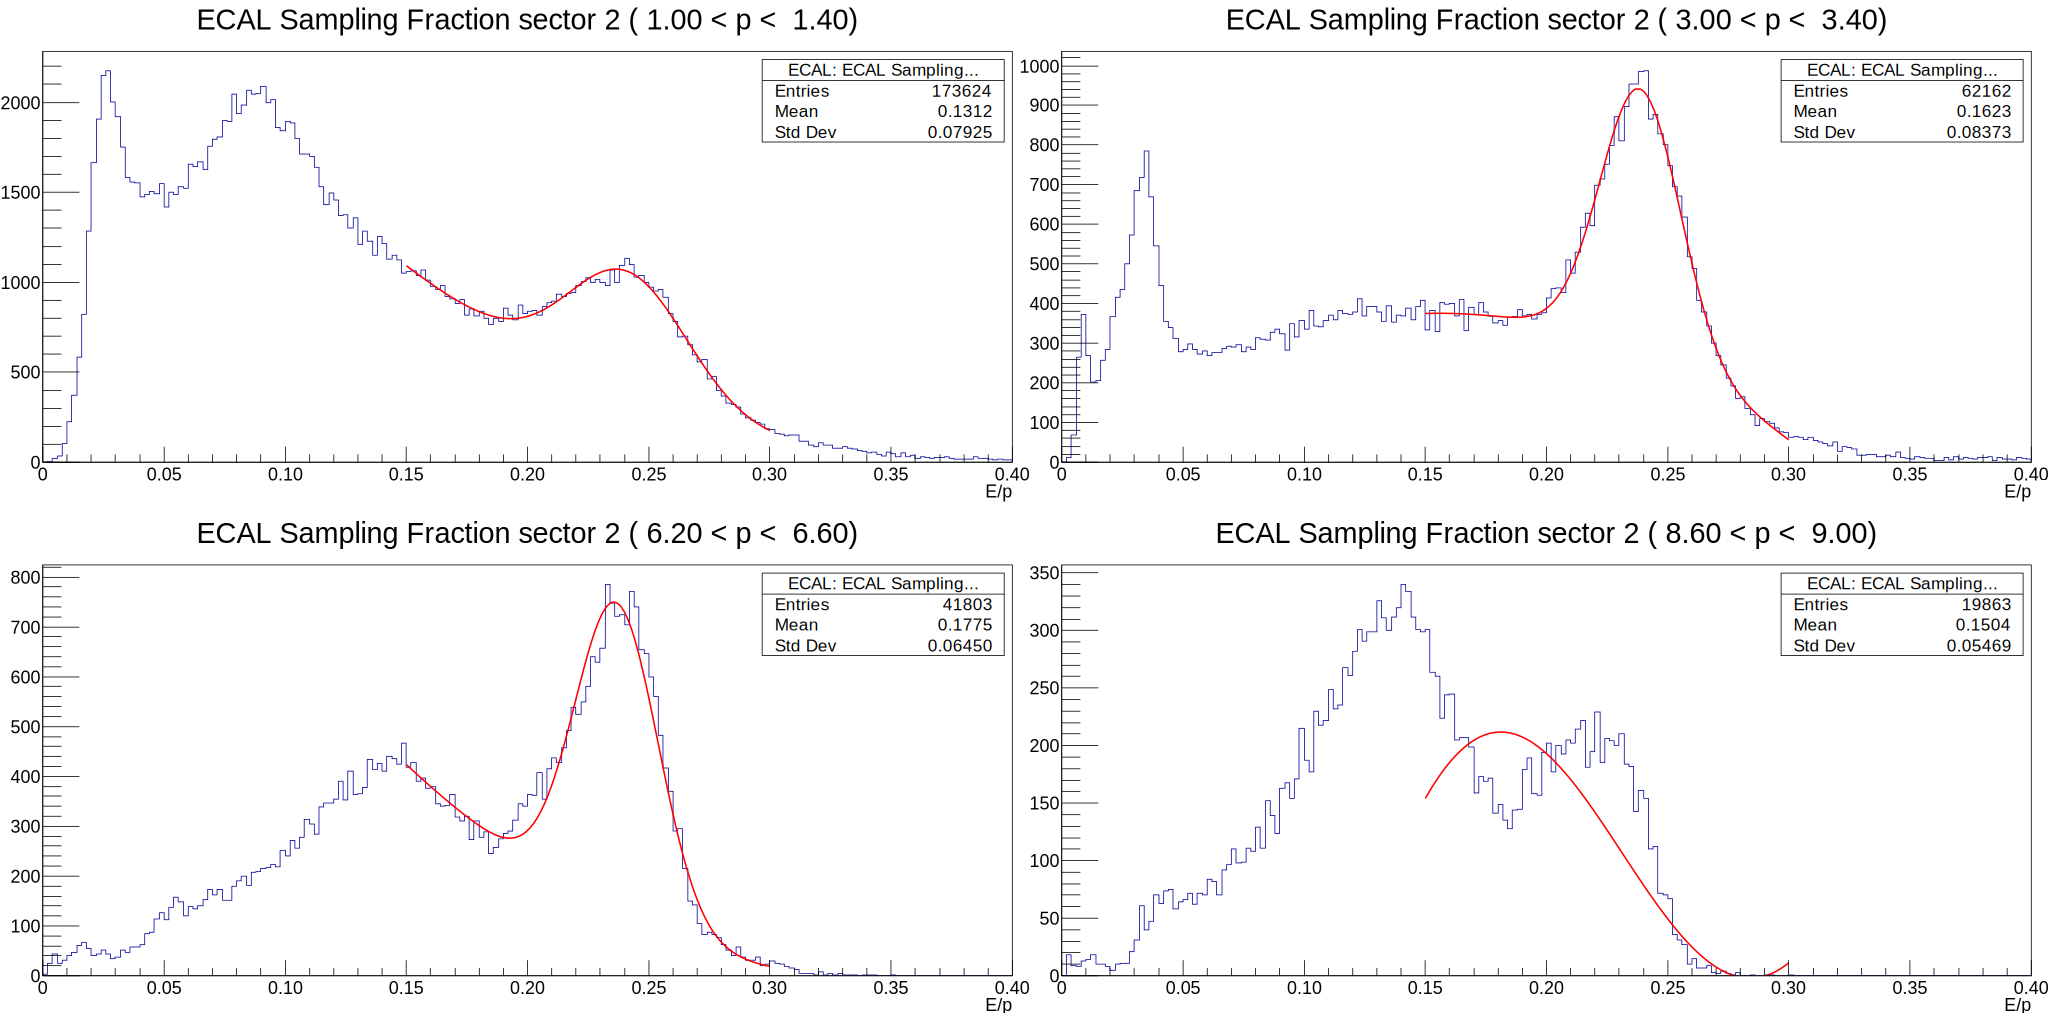
\includegraphics[width=\textwidth]{13dataanalysis/img/30sf_1d_plots.pdf}}
        \caption[Calorimeters $E/p$ plots]{Four $E/p$ plots describing the sum of the deposited energy per particle on all calorimeters (PCAL, ECIN, and ECOU). The particles' momentum is obtained from tracking and the event builder. As can be seen in the northwest and the southeast plots, the corner bins -- $1.00$ to $1.40$ and $8.60$ to $9.00 [\text{GeV}]$ respectively -- are not very reliable.}
        \label{fig::sf_1d}
    \end{figure}

\subsection{Sampling Fraction} \label{ssec::sampling_fraction}
    The energy deposited by electrons in the active area of the calorimeters is a fraction of their total energy $E_\text{tot}$.
    This value is proportional to their momentum $P$ for energies above a few hundred MeV.
    Heavier particles, due to their reduced penetration capabilities, tend to lose an amount of energy independent from their momentum.
    An electron sampling fraction measures the amount of energy lost depending on the momentum of a particle.
    This allows both the measurement of the electron's energy and the differentiation of electrons from other particles \cite{wigmans2000}.

    % Explain how the executable extracts the sampling fraction.
        % Show plot with curve of means!
    To obtain the sampling fraction, the hits of each calorimeter by itself (PCAL, ECIN, and ECOU) are separated in arrays, with an additional array containing the union of the three others.
    Then, these arrays of hits are separated into 20 momentum bins.
    Each bin has a size of $0.4 [\text{GeV}]$, starting at $1.0 [\text{GeV}]$ and ending at $9.0 [\text{GeV}]$.

    1-dimensional histograms are then drawn from the data in these arrays, measuring deposited energy divided by vertex momentum ($E/p$).
    A Gaussian fit plus quadratic background is then applied, as described by the following function:
    \begin{equation*}
        f(x) = p_0 g(x, \mu, \sigma) + p_1 x^2 + p_2 x + p_3, \hspace{12pt}
        \text{where} \hspace{4pt}
        g(x, \mu, \sigma) = \frac{1}{\sigma \sqrt{2\mu}} \exp \left(-\frac{1}{2} \frac{(x - \mu)^2}{\sigma^2}\right),
    \end{equation*}
    where $\mu$ and $\sigma$ are the mean and standard deviation of the distribution, respectively.
    Since the expected range of deposited energy $E/p$ expected for electrons is between $0.15$ to $0.30$ from theory, the fit is limited to that range.

    Examples of these plots are given in figure \ref{fig::sf_1d}.
    As can be seen in the figure, not enough electrons are seen in extreme momentum ranges, like from $1$ to $1.4$ GeV or from $8.6$ to $9$ GeV.
    Due to this, the sampling fraction fit described later only considers data in the range from $1.4$ to $8.6$ GeV.

    The mean of each of these fits is then extracted to be used as data points for a sampling fraction fit.
    A polynomial fit is used, since it follows well the shape of these points, and is what's used in the reconstruction software.
    The fit described by
    \begin{equation*}
        f(x) = p_0 \cdot \left(p_1 + \frac{p_2}{x} + \frac{p_3}{x^2}\right),
    \end{equation*}
    The $E/p$ distribution vs $p$ is shown in figure \ref{fig::sf_2d} along with this fit.

    \begin{figure}[t!]
        \centering\frame{
        \includegraphics[width=\textwidth]{13dataanalysis/img/30sf_2d_plot.pdf}}
        \caption[Calorimeters $p vs E/p$ plots]{A 2d plot showing momentum $p$ vs deposited energy divided by momentum $E/p$. The particle's deposited energy on all calorimeters is measured. Its momentum is obtained from tracking and the event builder. The fit follows the deposited energy of electrons to find their sampling fraction.}
        \label{fig::sf_2d}
    \end{figure}

    Finally, the parameters of the fit are stored in plain text files, following the convention in the CCDB.
    The parameters obtained can later be used to perform particle identification for electrons and photons.
    In addition, they are used to obtain the energy of electrons and photons since, as mentioned before, not all of it is deposited in the calorimeters.
